\documentclass[10pt,a4paper]{article}
\usepackage[utf8]{inputenc}
\usepackage{amsmath}
\usepackage{amsfonts}
\usepackage{amssymb}
\usepackage{amsthm}
\usepackage{graphicx}
\usepackage[margin=0.6in]{geometry}
\setcounter{section}{1}
\begin{document}



\section*{\textit{Prüfungsrelevante} Verfahren, Sätze und Rechenregeln}
\section{Diskrete Strukturen}
\subsection{Mengenlehre und Kombinatorik}
\begin{itemize}
\item zwei Mengen $A$ und $B$ sind gleich wenn sie die selben Elemente haben, d.h. wenn $A \subseteq B \land B \subseteq A$
\item Beachte z.B. dass $\left\lbrace\left\lbrace 1,2\right\rbrace, 7\right\rbrace \nsubseteq \mathbb{N}$
\item Schnitt und Vereinigung sind kommutativ, assoziativ, distributiv in beide Richtungen; für Beweise kann es nützlich sein sich die Definitionen dieser Operationen in Erinnerung zu rufen; $\overline{A\cup B}=\overline{A}\cap \overline{B}, \overline{A\cap B}=\overline{A}\cup \overline{B}$
\item $A\times B=\left\lbrace (a,b)\mid a\in A \land b\in B\right\rbrace$ heißt \textbf{kartesisches Produkt} oder \textbf{Produktmenge};  $\vert A\times B\vert =\vert A\vert \cdot \vert B\vert$
\item \textbf{Potenzmenge} $\mathcal{P}(A)$ ist die Menge aller (auch unechten) Teilmengen von $A$, $\vert \mathcal{P}(A)\vert =2^{\vert A\vert}$, es gilt stets $\emptyset \in \mathcal{P}(A)$
\item $\begin{pmatrix} n\\ k\end{pmatrix}=\dfrac{n!}{k!(n-k)!}=\begin{pmatrix} n\\ n-k\end{pmatrix};\;\;\begin{pmatrix} n+1\\ k\end{pmatrix}=\begin{pmatrix} n\\ k-1\end{pmatrix}+\begin{pmatrix} n\\ k\end{pmatrix}$
\item \textbf{Handschlaglemma:} Anzahl der Teilnehmer einer Konferenz, die einer ungeraden Anzahl von Teilnehmern die Hand geben, ist immer gerade

%genauer siehe Graphentheorie, ich hab versucht da eine Form zu finden die man sich besser merken kann aber das scheint tatsächlich nur in der Graphentheorie eine größere Rolle zu spielen; daher zeile evtl. noch zu streichen 

\end{itemize}



\subsection{Abbildungen}
\begin{itemize}
\item für $f: A\rightarrow B, A'\subseteq A$ heißt $f[A']=\left\lbrace f(a)\mid a \in A'\right\rbrace$ Bild von $A'$ unter $f$
\item \textbf{injektiv:} $f(a_{1})=f(a_{2}) \Rightarrow a_{1}=a_{2}$ ("für jedes $b\in B$ existiert höchstens ein $a\in A$ mit $f(a)=b$")\\
Beweise über Gegenbeispiel oder $f(a_{1})=f(a_{2})$ setzen 
\item \textbf{surjektiv:} $f[A]=B$ ("für jedes $b\in B$ existiert mindestens ein $a\in A$ mit $f(a)=b$")\\ Beweise über Gegenbeispiel oder Definitionsbereich der Umkehrfunktion untersuchen 
\item \textbf{bijektiv:} injektiv und surjektiv ("für jedes $b\in B $ existiert genau ein $a\in A$ mit $f(a)=b$")
\item für $f$ \textit{injektiv (!!)}  definieren wir $\boldsymbol{f^{-1}: }f[A]\rightarrow A, b\mapsto f^{-1}(b)=a$ mit $f^{-1}(b)=a$  g.d.w. $f(a)=b$
\item für $f:A\rightarrow B, g: B\rightarrow C$ ist \textbf{Komposition} $ g\circ f:A\rightarrow C, x \mapsto g(f(x))$ ($\Rightarrow$ von rechts nach links ausführen!!)
\end{itemize}



\subsection{Permutationen}
\begin{itemize}
\item \textbf{Permutation} von $X$ ist bijektive Abbildung von $X$ nach $X$, für $X=\left\lbrace 1,\dotsc, n\right\rbrace$ ist $S_{n}$ Menge aller Permutationen und $\pi \in S_{n}$ mit $\pi=\begin{pmatrix}1&\dotsc& n\\ \pi(1)&\dotsc &\pi(n)\end{pmatrix} $ und $\vert S_{n}\vert =n!$
\item \textbf{k-Zyklus} = k-Tupel der Form $(a_{1},\dotsc,a_{k})$ mit $\pi(a_{k})=a_{1}, \pi(a_{i})=a_{i+1}$, jedes Element von $S_{n}$ kann als Komposition elementfremder Zyklen notiert werden: $\begin{pmatrix}1&2& 3&4&5\\ 2&3&1&5&4\end{pmatrix}=(1,2,3)\circ (4,5)=(123)(45)$
\item bei elementfremden Zyklen ist Reihenfolge egal: $(123)(45)=(45)(123)$; Elemente die auf sich selbst abgebildet werden heißen \textbf{Fixpunkte} und müssen nicht notiert werden: $(123)(4)=(123)$; mit welchem Element im Zyklus angefangen wird ist Egal: $(123)(45)=(312)(54)$ 
\item \textbf{Transposition} = 2-Zyklus, jedes Element von $S_{n}$ kann mit Transpositionen geschrieben werden als:\\ $(a_{1}\dotsc a_{k})=(a_{1}a_{2})(a_{2}a_{3})\dotsc(a_{k-1}a_{k})$ (nicht elementfremd $\Rightarrow$ Reihenfolge wichtig!!)
\item bei Komposition von Permutationen für jede Zahl von rechts nach links durchgehen: $\underbrace{(123)}_{\text{\textit{(2)}}}\underbrace{(35)}_{\text{\textit{(1)}}}=\underbrace{(1235)}_{\text{\textit{(3)}}}$\\5 wird in \textit{(1)} auf 3 abgebildet, in \textit{(2)} wird 3 auf 1 abgebildet, also $5\rightarrow 3 \rightarrow 1$ und damit $5\rightarrow 1$  in \textit{(3)} 
\item für $\alpha=(125)(38)(47)$ ist ord$(\alpha)=\text{kgV}(\underbrace{3,2,2}_{\text{ord der Zyklen}})=6\Rightarrow \alpha^{6}=\text{id}_{X} \Rightarrow \alpha^{5}=\alpha^{-1}, \alpha^{n}=\alpha^{n \mod 6}$\\
für $\alpha^{-1}$ kann man auch einfach Zeilen vertauschen
\end{itemize}



\subsection{Beweis mittels vollständiger Induktion (Beispiel)}
\textit{Beweis.}
Die Aussage $A_{n}$ sei $\sum_{k=0}^{n} q^{k}= \dfrac{1-q^{n+1}}{1-q}$ mit $n \in \mathbb{N}, q \in \mathbb{R}, q \neq 1$.\\\\
(IA): $n_{0}=0$: $\sum_{k=0}^{0} q^{k}=q^{0}=1= \dfrac{1-q^{0+1}}{1-q}$ \hspace{0.3cm} w.A.\\
\hspace*{1cm}$\Rightarrow$ Es gilt $A_{0}$\\\\
(IV): $\forall \tilde{n}: n_{0} \leq \tilde{n} \leq n:\sum_{k=0}^{\tilde{n}} q^{k}= \dfrac{1-q^{\tilde{n}+1}}{1-q}$\\\\
(IS):$\sum_{k=0}^{n+1} q^{k}= \sum_{k=0}^{n} q^{k}+q^{n+1}\stackrel{\text{(IV)}}{=}\dfrac{1-q^{n+1}}{1-q}+q^{n+1}=\dfrac{1-q^{n+1}+(1-q)q^{n+1}}{1-q}$\\
\hspace*{2.23cm}$=\dfrac{1-q^{n+1}+q^{n+1}-q^{n+2}}{1-q}=\dfrac{1-q^{(n+1)+1}}{1-q}$\\\\
\hspace*{1cm}$\Rightarrow$ Damit ist die Behauptung für alle $n \in \mathbb{N}$ vollständig bewiesen
\qed\\\\
\begin{itemize}
\item "Die Aussage $A_{n}$ sei..." nur in VL und AuD Skript, \textit{evtl.} wird sonst aber z.Z.: erwartet; IV muss auch nicht unbedingt notiert werden
\item alles nochmal mit (n+1)+1 hinschreiben ist nicht nötig
\item Varianten: $A_{n} \Rightarrow A_{n+1}$/ aus $A_{n}$ folgt $A_{n+1}$ für alle $n\in \mathbb{N}$\\
 w.A. /Folglich gilt $A_{n}$ für alle $n \in \mathbb{N}, n \geq n_{0}$
\item Beachte dass oft auch nur für $n \in \mathbb{N}, n\geq k$ bewiesen wird (kein $\tilde{n}$)!! und $n_{0}=0$ nicht immer gelten muss
\end{itemize}



\subsection{Zahlentheorie}
\begin{itemize}
\item $n\in \mathbb{N}, n\geq 1$ kann \textit{eindeutig} geschrieben werden als $n=\prod_{i=1}^{k} p_{i}^{\alpha_{i}}$ ($p_{i}$ prim, $\alpha_{i} \in \mathbb{N},$ "PFZ")\\ $\Rightarrow\#\text{Teiler von }n=\prod_{i} (\alpha_{i}+1)$
\item für $a,b \in \mathbb{N}$ gilt $a\mid b \Leftrightarrow \exists k :k\in\mathbb{N}\land  ak=b;\;\;\; a\mid b_{1}\land a\mid b_{2} \Rightarrow a\mid (b_{1}+b_{2}) \land a\mid (b_{1}-b_{2})$
\item für $m,n \in \mathbb{Z}$ mit $n>0$ gilt $\exists q,r:( q,r \in \mathbb{Z}\land m=nq+r\land 0\leq r<n)$\\ $m \text{ mod } n:=r,\;\;$
für $a \text{ mod } n =b \text{ mod } n$ schreibe $a \equiv b \text{ mod } n$
\item \textbf{Homomorphieregel:} $(a \text{ mod } n+b \text{ mod } n) \text{ mod } n=(a+b) \text{ mod } n\;\;\;\;\;$ (analog für $\cdot\;$)
\item $\text{kgV}(m,0)=\text{kgV}(0,n)=0;\;\text{ggT}(m,n)\cdot \text{kgV}(m,n)=m\cdot n\;(\Rightarrow$ kgV mit Euklid berechenbar) 
\item \textbf{Euklidischer Algorithmus:}
für $m,n\in\mathbb{N},m\leq n$!!, immer weiter ggT$(m,n)=\text{ggT}(n \text{ mod } m,m)$ berechnen; $\;\text{ggT}(m,n)=m$ falls $m\mid n;\;\; \text{ggT}(0,n)=n;\;\; m,n \text{ teilerfremd }  \Leftrightarrow \text{ggT}(m,n)=1$
\item \textbf{Lemma von Bézout:} $m,n \in \mathbb{N} \Rightarrow \exists a,b :a,b\in \mathbb{Z}\land \text{ggT}(m,n)=am+bn\;\;$ ($a,b$ nicht eindeutig)
\item \textbf{Erweiterter Euklidischer Algorithmus} am Beispiel ("EEA", keine offizielle Abkürzung): \\
\end{itemize}
\begin{tabular}{ c | c c | c }
   & $\underbrace{1008}_{m}$ & $\underbrace{499}_{n}$ & $-q_{i}$ \\ 
 \hline
 1008 & 1 & 0 & \\  
 499 & 0 & 1 &  \\  
$1008 \text{ mod } 499 =10$ & 1 & $0+1\cdot(-q_{i})=-2$ & $1008=499\cdot 2+10\Rightarrow -q_{i}=-2$\\
$499 \text{ mod } 10 =9$ & -49 & $1+(-2)(-q_{i})=99$ & $499=10\cdot 49+9\Rightarrow -q_{i}=-49$  \\
$10 \text{ mod } 9= \underbrace{1}_{\text{ggT}}$ & 50 & $-2+99(-q_{i})=-101$ & $10=9\cdot 1+1\Rightarrow -q_{i}=-1$ \\
$9 \text{ mod } 1 =0$&STOP&&
\end{tabular} 
\hspace{0.1cm} $\Rightarrow$\hspace{0.2cm}
\begin{tabular}{ c | c c | c }
   & 1008 & 499 & $-q_{i}$ \\ 
 \hline
 1008 & 1 & 0 & \\  
 499 & 0 & 1 &  \\  
 10 & 1 & -2 & -2\\
 9 & -49 & 99 & -49  \\
 1 & 50 & -101 & -1 \\
\end{tabular} \\\\\\
in $m$ Spalte wird analog zu $n$ Spalte gerechnet; EEA für $m,n\in\mathbb{Z}$: mit $\vert m\vert,\vert n\vert $ rechnen, dann Ergebnis anpassen\\
$\Rightarrow \text{ggT}(1008,499)=1=50\cdot 1008 -101\cdot 499\;\;\;\;\;$ (Bézout Koeffizienten $a=50, b=-101$)
\begin{itemize}
\item \textbf{chinesischer Restsatz:} Seien $0<n_{1},\dotsc ,n_{k}\in \mathbb{N}$ teilerfremd und seien $a_{1},\dotsc ,a_{k} \in \mathbb{Z}$. Dann existiert genau ein $x\in \left\lbrace 0,1,\dotsc,\prod_{i=1}^{k} n_{i}-1\right\rbrace$ mit $x\equiv a_{i} \text{ mod } n_{i}$ für alle $i=1,\dotsc, k$
\item für $k=2:$ Seien $0<m,n\in \mathbb{N}$ teilerfremd und seien $a_{1},a_{2} \in \mathbb{N}$. Dann existiert genau ein $x\in \left\lbrace 0,1,\dotsc,mn-1\right\rbrace$ mit $x\equiv a_{1} \text{ mod } m \land x\equiv a_{2} \text{ mod } n;\;$ anschaulich heißt das, dass ein $m\times n$ Spielbrett eindeutig wie in VL durchnummeriert werden kann wenn $\text{ggT}(m,n)=1$

%warum $a_{1},a_{2} \in \mathbb{N}$, nicht $\mathbb{Z}$??

\end{itemize}




\subsection{Gruppentheorie}
\begin{itemize}
\item Gruppe $(G,\circ)$ (auch $(G;\circ,^{-1},e)$; dann Definition einfach anders formulieren) besteht aus Menge $G$ und innerer Verknüpfung $\circ:G\times G\rightarrow G$, so dass: $\circ$ assoziativ, es existiert  \textbf{neutrales Element} $e\in G$ ($a\circ e=a=e\circ a$ für alle $a\in G$), es existiert \textbf{Inverses} $a^{-1}\in G$ zu jedem $a\in G$ (mit $a\circ a^{-1}=e=a^{-1}\circ a$)
\item beweisen, dass es sich um eine Gruppe handelt z.B. per Tabelle möglich, oft kann man auch argumentieren dass Eigenschaften wie Assoziativität geerbt werden
\item Gruppe heißt \textbf{abelsch}/kommutativ, falls $\circ$ kommutativ ist
\item $\mathbb{Z}_{n}=\left\lbrace 0,\dotsc,n-1\right\rbrace $ bildet mit Addition mod $n$ eine Gruppe; Menge aller Permutationen auf einer Menge kann als Gruppe aufgefasst werden, z.B. Eckenpermutationen eines Quadrates ("$D_4"/"D_{8}"$)(Komposition führt zu Drehungen, Spiegelungen und Identitätsabbildung)
\item \textbf{Nullteiler} mod $n$ sind $a\in \mathbb{Z}_{n}\setminus \left\lbrace 0\right\rbrace$ für die $b\in \mathbb{Z}_{n}\setminus \left\lbrace 0\right\rbrace$ existiert mit $a\cdot b\equiv 0 \text{ mod } n$\\
\textbf{Einheiten} mod $n$ sind $a\in \mathbb{Z}_{n}$ für die $b\in \mathbb{Z}_{n}$ existiert mit $a\cdot b\equiv 1 \text{ mod } n$, 1 ist immer eine Einheit\\
$m$ ist Einheit mod $n\Leftrightarrow$ $m$ ist kein Nullteiler mod $n\Leftrightarrow$ ggT$(m,n)=1$
\item Die Menge der Einheiten mod $n$ heißt $\mathbb{Z}_{n}^{*}$ und bildet eine Gruppe mit Multiplikation mod $n$; es gilt mit PFZ, dass $\phi(n):=\vert \mathbb{Z}_{n}^{*}\vert=\prod_{i=1}^{k}(p_{i}^{\alpha_{i}}-p_{i}^{\alpha_{i}-1})=\# \text{ zu } n \text{ teilerfremde Zahlen die kleiner (-gleich) }n \text{ sind}$
\item eine multiplikative Gruppe ist \textbf{zyklisch}, falls $g\in G$ existiert mit $G=\left\lbrace g^{j}\mid j \in \mathbb{Z}\right\rbrace$, ein solches $g$ heißt \textbf{Erzeuger} von $G$ (Potenzrechengesetze ähnlich wie in $\mathbb{N}$, für additive Gruppen schreibe $G=\left\lbrace jg\mid j \in \mathbb{Z}\right\rbrace$); für Erzeuger gilt mit $\vert G\vert=n$, dass $G=\left\lbrace g^{j}\mid j \in \mathbb{Z}_{n}\right\rbrace;$
\item Erzeuger von $(\mathbb{Z}_{n},+ \mod n)$ sind genau die Elemente von $\mathbb{Z}_{n}^{*}\Rightarrow$ \# Erzeuger$=\phi(n)$ 
\item Ein \textbf{Satz von Gauß}: für $p$ prim ist $(\mathbb{Z}_{p}^{*}, \cdot \text{ mod } n$) zyklisch; \# Erzeuger$=\phi(p-1)=\phi(\phi(p))$; diese Erzeuger heißen \textbf{Primitivwurzeln}
\item "Finden Sie Erzeuger/Primitivwurzel/ist $G$ zyklisch?": i.A. Tabelle erstellen ($n=\vert G\vert$ )
\begin{tabular}{c|c c c}
$n$ & 2&$\cdots$ &$n$\\
\hline
$g_{1}^{n}$&&&\\
$\vdots$ &&&\\
$g_{n}^{n}$&&&
\end{tabular}

sobald man für $j\neq0$ auf $g^{j}=1$ kommt kann man aufhören (da gilt $j\in \mathbb{Z}_{n}$ und damit immer schon $1=g^{0}$)
\item Inverses zu Einheit $g$ von $\mathbb{Z}_{n}$ berechnen: EEA$(n,g)\Rightarrow 1=ag+bn\Rightarrow 1\equiv ag \mod n$\\
Achtung: evtl. ist $a\notin \mathbb{Z}_{n}$!!! (z.B. weil $a$ negativ $\Rightarrow g^{-1}=n-a$)
\item \textbf{isomorph}=Strukturgleich ("man kann Elemente einfach umbenennen"), jede zyklische Gruppe ist isomorph entweder zu $(\mathbb{Z},+)$ oder einem $(\mathbb{Z}_{n},+ \text{ mod } n)$; als Beweis das zwei Gruppen nicht isomorph sind genügt z.B. "$G_{1}$ ist zyklisch, $G_{2}$ nicht "
\item $U\subseteq G$ heißt \textbf{Untergruppe} von $G$ falls $e\in U;\;\; a\circ b \in U \text { für alle } a,b\in U;\;\; a^{-1} \in U \text{ für alle } a \in U$ 
\item $\langle g \rangle:=\left\lbrace g^{i}\mid i \in \mathbb{Z}\right\rbrace$ ist \textbf{von $\boldsymbol{g}$ erzeugte Untergruppe}
\item $g \circ U=\left\lbrace g\circ u \mid u \in U \right\rbrace$ ist eine \textbf{(Links-)Nebenklasse} ("LNK") von $U,\; \vert g\circ U\vert =\vert U\vert$, 2 LNK sind entweder gleich oder disjunkt $\Rightarrow$ jedes $g\in G$ liegt in genau einer LNK (nämlich $g\circ U$)
\item \textbf{Satz von Lagrange:} $\vert G \vert = \vert G : U \vert \cdot \vert U \vert\;\;\;\;$  ( $\vert G : U \vert=\#$ LNK von $U$ in $G$=Index von $U$ in $G$)\\ $\vert G \vert$ heißt Ordnung von $G$, o$(g):=\vert \langle g\rangle \vert$ Ordnung von $g$; $g^{\vert G\vert}=e$
\item "Finden Sie alle $\langle g \rangle$": ausnutzen welche Werte für o$(g)$ nach Lagrange nur möglich sind \\
"Finden Sie Untergruppen der Ordnung 2/3": $U_{2}$ enthält nur 1 und $g$ mit $g^{2}=1$, $U_{3}$ enthält nur 1 und $g_{1},g_{2}$ mit $g_{1}^{2}=g_{2},g_{2}^{2}=g_{1}$ ($\Rightarrow$  beides per Verknüpfungstafel lösbar)
\item "Finden Sie die LNK von $U$": per Verknüpfungstafel rechnen, ausnutzen dass LNK gleich oder disjunkt sind
\item \textbf{Satz von Euler-Fermat:} Seien $n\in \mathbb{N}, a\in \mathbb{Z}$ mit ggT$(a,n)=1$. Dann gilt $a^{\phi(n)}\equiv 1 \text{ mod } n$. (bei kleinem Fermat gilt $n$ prim)
\item für Beweise bieten sich oft Verknüpfungstafeln an, folgende Methoden helfen beim effizient rechnen: Kongruenz mit kleineren negativen Zahlen ausnutzen, für $\circ$ kommutativ ist Tafel symmetrisch bzgl. Hauptdiagonale, Sudokuprinzip (jede Zahl nur ein mal pro Zeile/Spalte)
\item dass ggT$(m,n)\geq 2$ kann man auch damit begründen, dass $m,n$ beide z.B. 2 in PFZ haben, für ggT von kleinen Zahlen ist keine Begründung nötig
\item Gleichungen in $\mathbb{Z}_{n}$: $\underline{123^{321}\cdot x\equiv}  3^{321(\mod \phi(40))}\cdot x\equiv 3x \equiv \underline{ 4 (\mod 40)}$, mit $3^{-1}=27$ folgt $x\equiv (27\cdot 4 )(\mod 40) $
\end{itemize}



\subsection{Effizient potenzieren mod $\boldsymbol{n}$}
\begin{itemize}

% al kashi würde ich nicht mitnehmen weil sehr umständlich und nicht ausdrücklich gefordert und wenn euler fermat nicht geht ist man mit zerlegen doch am ende genau so schnell

\item andere Form von Euler-Fermat: $a^{m} \equiv a^{m \text { mod } \phi (n)} \mod n\;\;$, gilt aber auch nur für ggT$(a,n)=1$ !!
\item einfach die Zahlen Stück für Stück mit mod zerlegen
\end{itemize}



\subsection{Kryptographie}
\begin{itemize}
\item für $p$ prim und $g$ Primitivwurzel von $\mathbb{Z}_{p}^{*}$ ist der \textbf{diskrete Logarithmus} von $x \in \mathbb{Z}_{p}^{*}$ zur Basis $g$ die Zahl $m\in \left\lbrace 0,\dotsc,p-2\right\rbrace$ mit  $g^{m}\equiv x \text{ mod } p\;\;\; (m=\text{log}_{g}(x))$; $m$ kann nicht effizient berechnet werden, $x$ aus $g^{m}$ schon
\item \textbf{Diffie-Hellman-Merkle:}
\begin{enumerate}
\item Alice und Bob einigen sich auf Primzahl $p$ und Primitivwurzel $g$ von $\mathbb{Z}_{p}^{*}$
\item Alice wählt geheime Zufallszahl $a$ und berechnet $a'=g^{a} \text{ mod } p$; Bob analog: $b'=g^{b} \text{ mod } p$
\item beide teilen sich $a'$ und $b'$ mit und berechnen das Geheimnis $c=g^{ab} \text{ mod } p=(a')^{b} \text{ mod } p=(b')^{a} \text{ mod } p$
\end{enumerate}
Um damit Nachricht $m\leq c$ zu verschlüsseln:
\begin{enumerate}
\item  schreibe $m$ und $c$ binär als $m=m_{1}\dotsc m_{l},c=c_{1}\dotsc c_{k}$
\item Alice verschickt $v_{1}=m_{1}+c_{1} \text{ mod } 2,\dotsc,v_{l}=m_{l}+c_{l} \text{ mod } 2$; Bob berechnet $m_{i}=v_{i}+c_{i} \text{ mod } 2$
\end{enumerate}
\item \textbf{RSA:}
\begin{enumerate}
\item Bob wählt zufällig 2 verschiedene Primzahlen $p,q$ und berechnet $n:=pq$
\item Bob wählt zufällig $d\in \mathbb{Z}_{\phi(n)}^{*}$ und berechnet $i,h\in \mathbb{Z}$ mit $ i\cdot d+h\cdot \phi(n)=\text{ggT}(d,\phi(n))=1$ (EEA)

%prüfen ob dieser Punk tatsächlich korrekt 

\item $n$ und $i$ sind öffentliche Schlüssel und werden an Alice weitergegeben, $d$ ist privater Schlüssel
\item Alice schickt $c=m^{i} \text{ mod } n$ an Bob mit Nachricht $m$ ($0\leq m <n$) 
\item Bob berechnet $m=c^{d} \text{ mod } n$ 
\end{enumerate}
\end{itemize}


\subsection{Ungerichtete Graphen}
\begin{center}
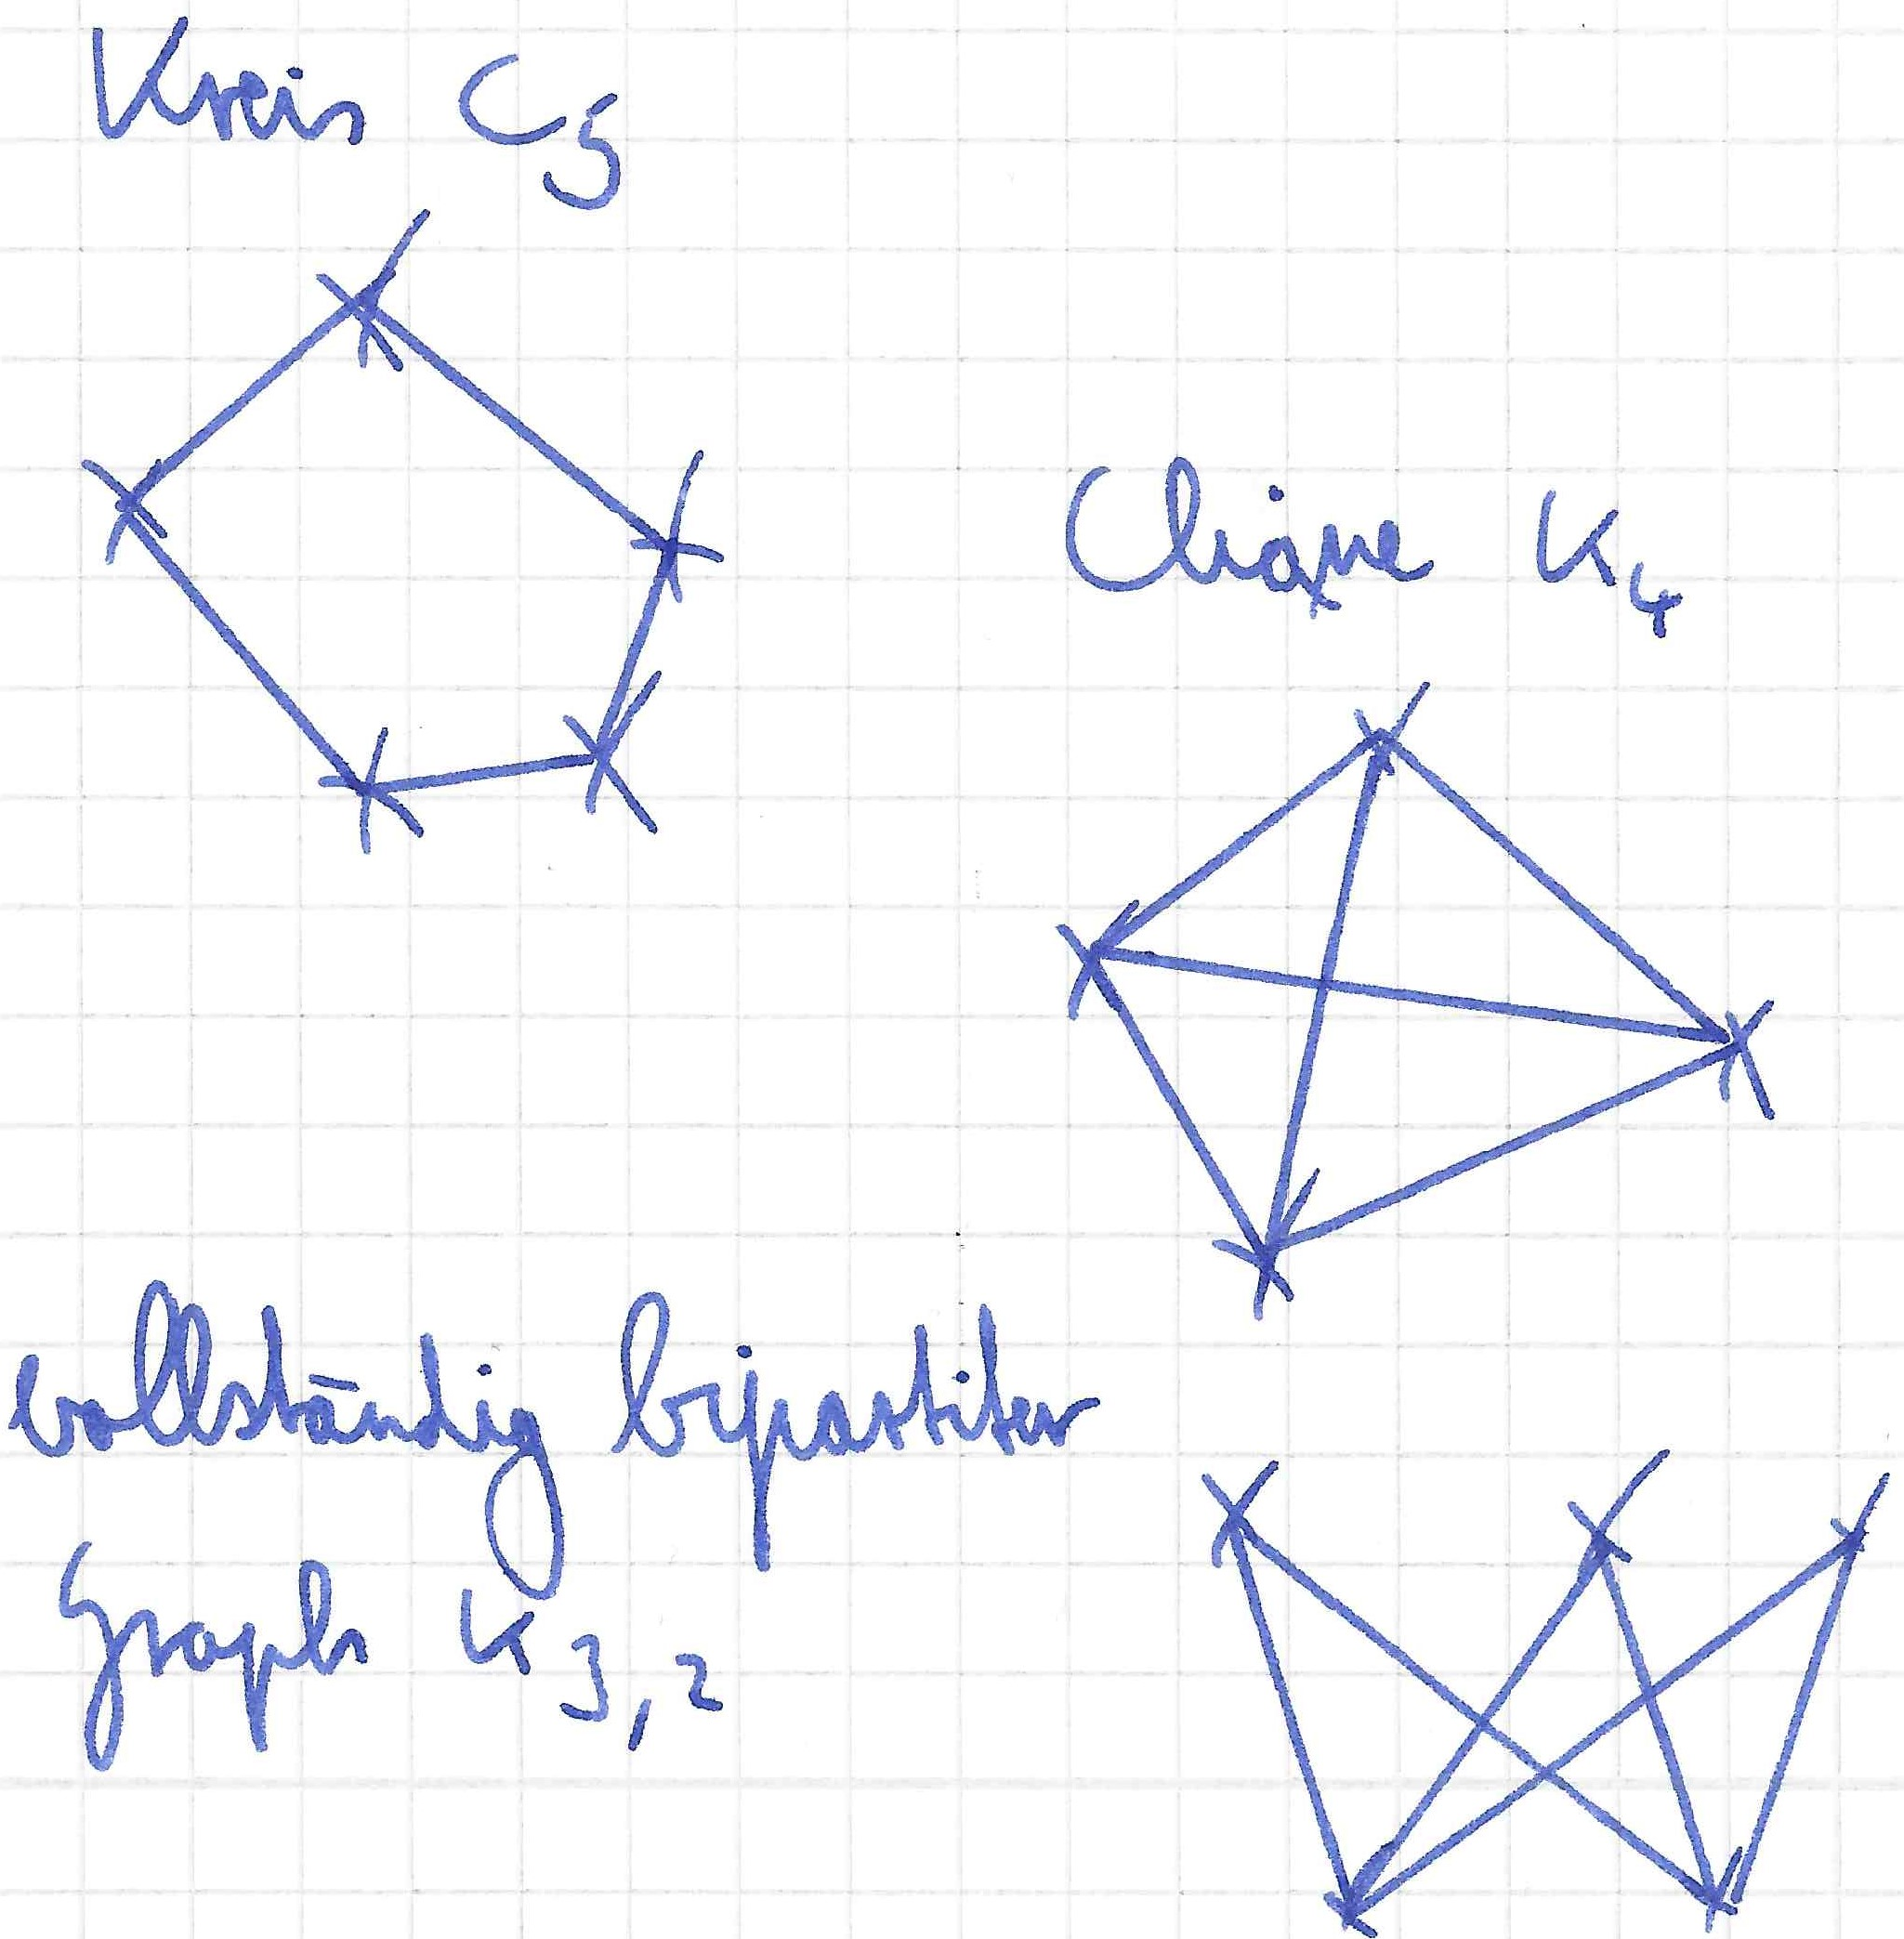
\includegraphics[scale=0.48]{typische_graphen.jpg} 
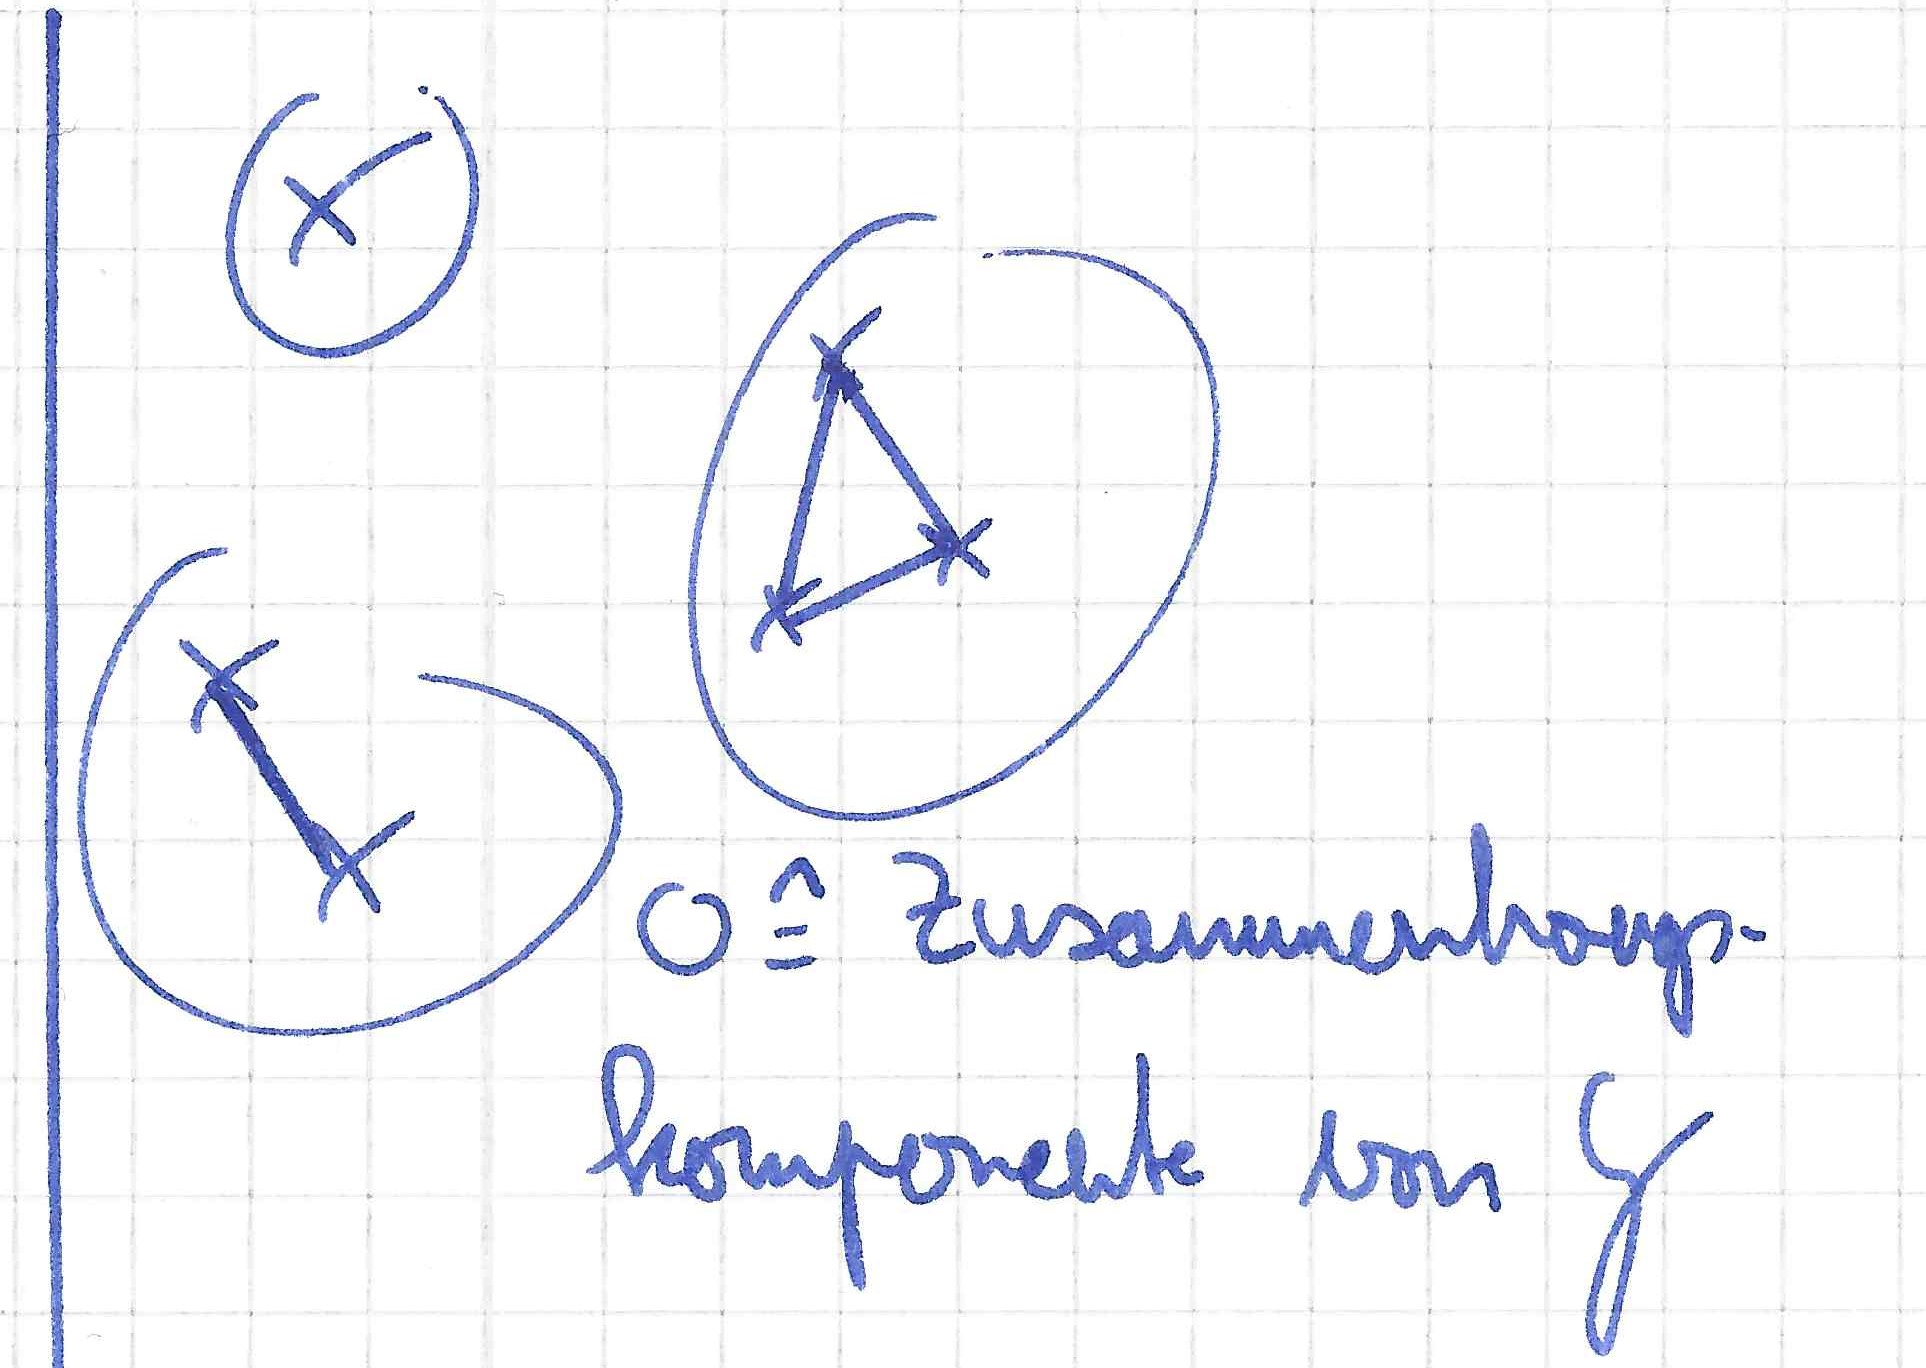
\includegraphics[scale=0.72]{zusammenhangskomponenten.jpg} 
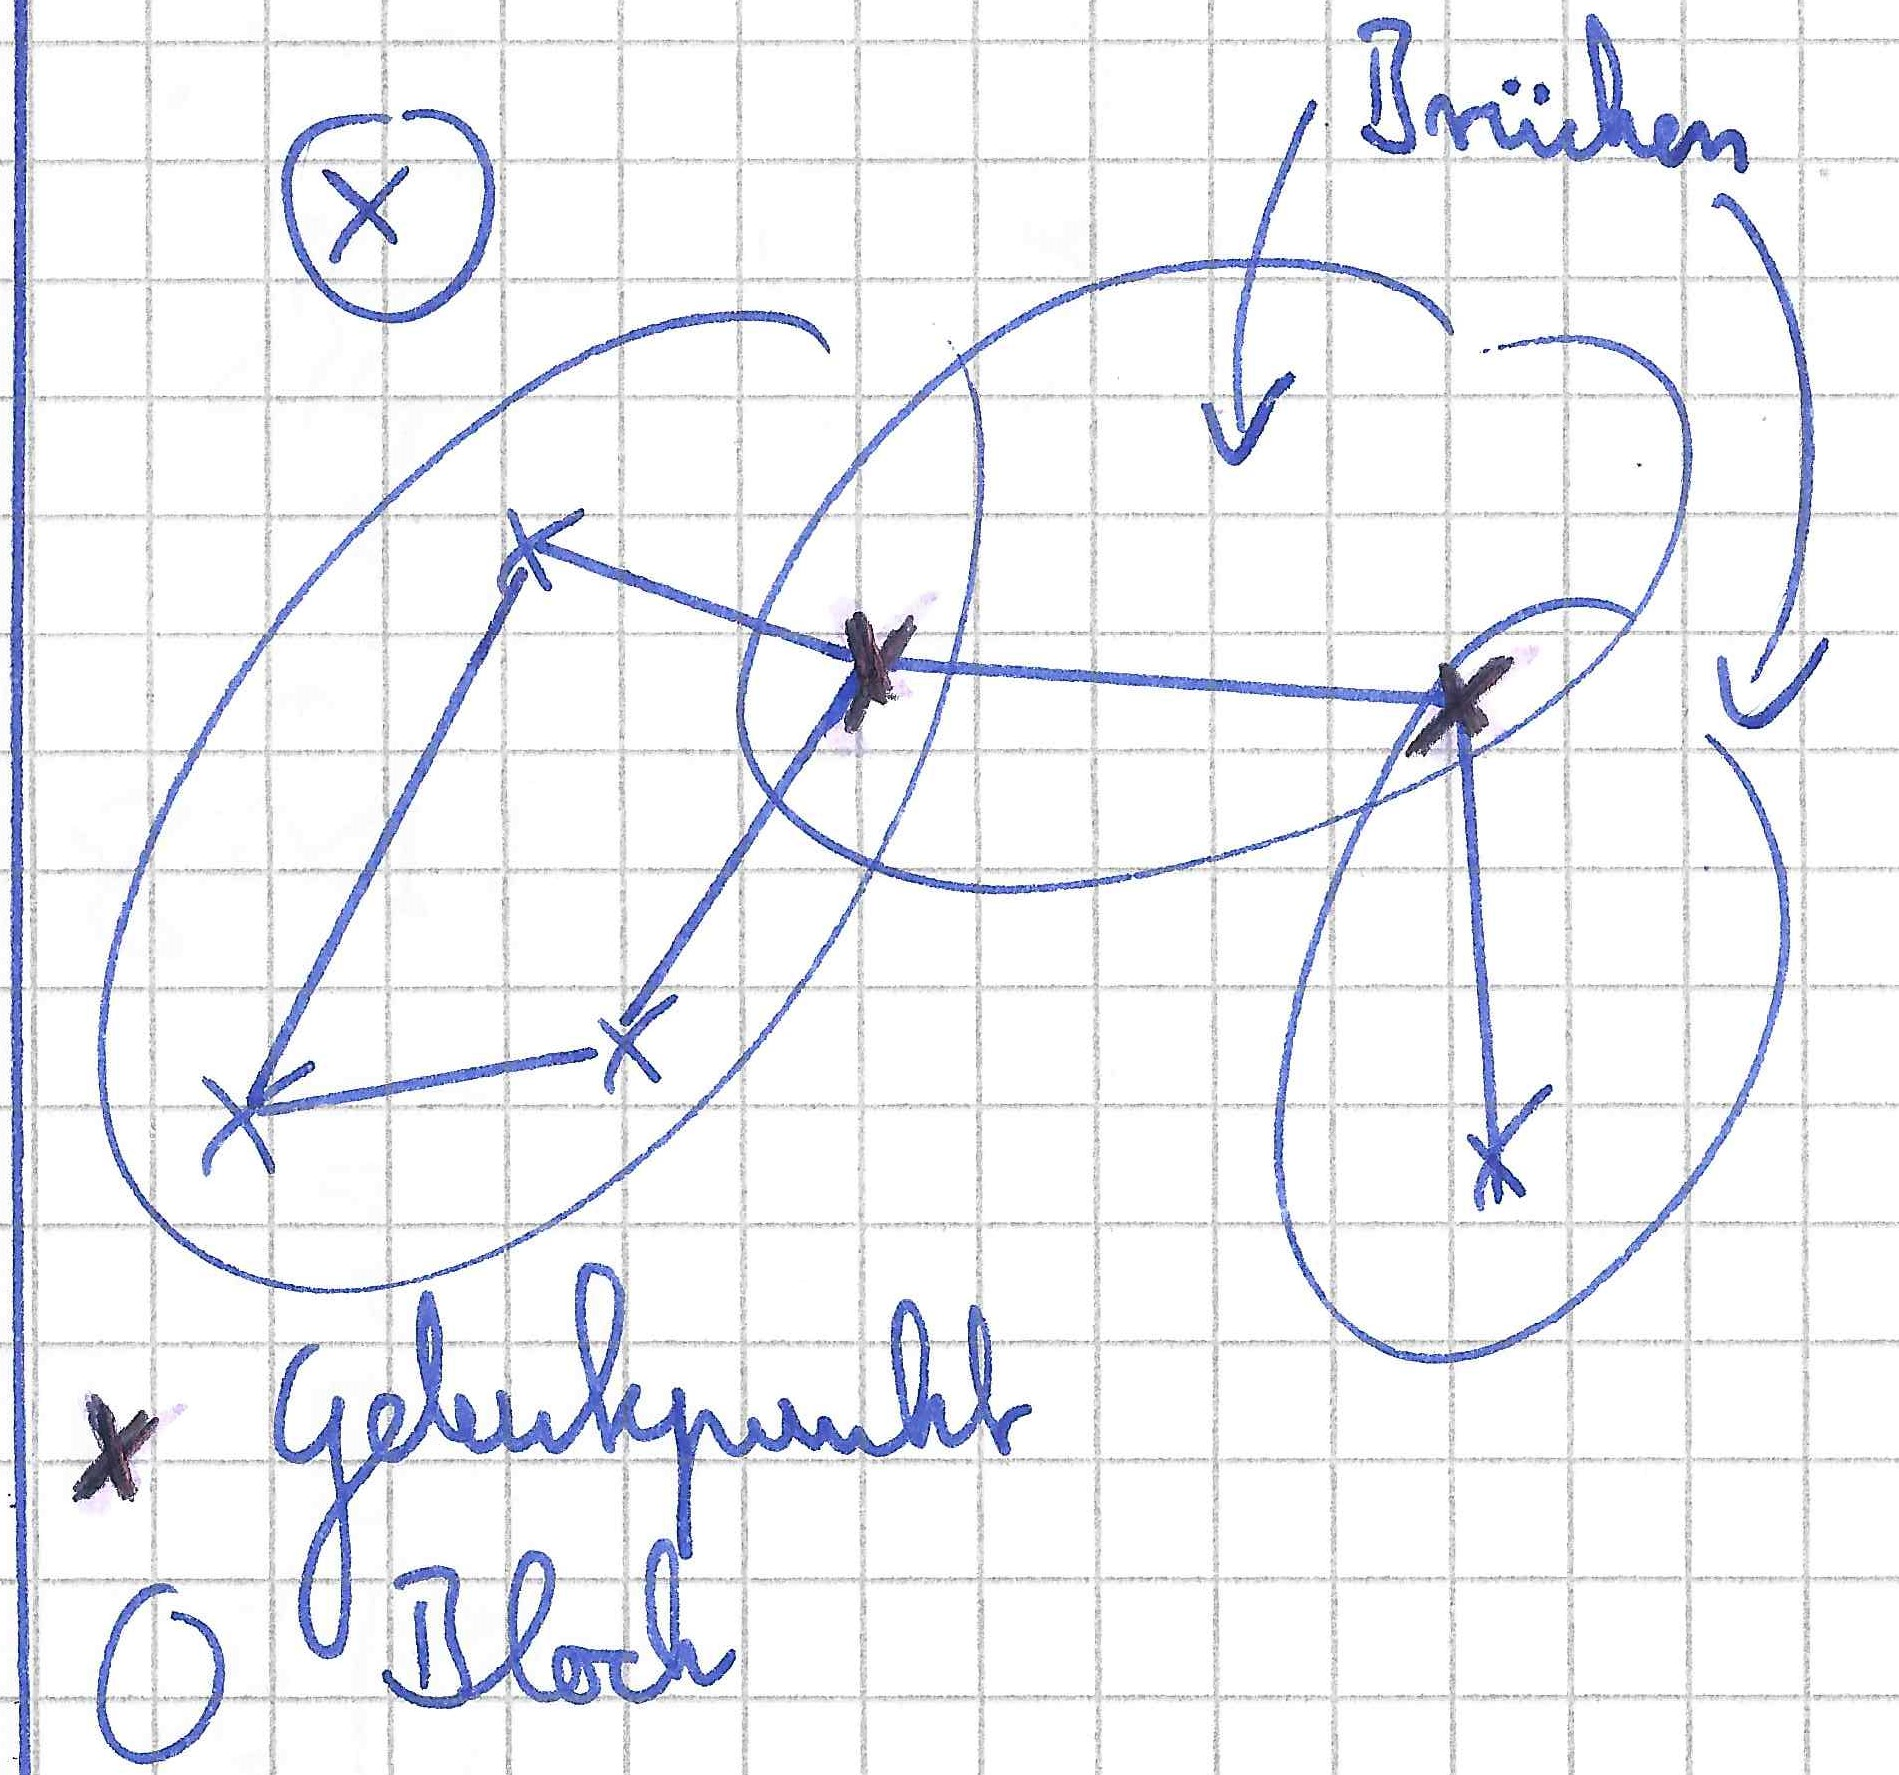
\includegraphics[scale=0.55]{bloecke.jpg} 
\end{center}

\begin{itemize}
\item \textbf{Komplementgraph} $\overline{G}:=\left(V,\begin{pmatrix}
V\\2
\end{pmatrix}\setminus E \right)\;\;\;\;$  (statt $\begin{pmatrix} V\\2 \end{pmatrix}$ scheint $\left\lbrace X \subset V : \vert X \vert=2\right\rbrace$ sicherer zu sein)
\item $G_{1}=(V_{1},E_{1}), G_{2}=(V_{2},E_{2})$ sind \textbf{isomorph}, wenn es eine Bijektion $f:V_{1}\rightarrow V_{2}$ gibt, so dass $\left\lbrace u,v\right\rbrace \in E_{1}$ g.d.w. $\left\lbrace f(u),f(v)\right\rbrace \in E_{2}$ für alle $u,v\in V_{1}.\;\;$(d.h. es muss auch gelten $\vert E_{1}\vert=\vert E_{2}\vert$)\\  ($G_{1}\cong G_{2}$)("sind $G_{1},G_{2}$ gleich wenn man die Knoten in $G_{2}$ umbenennt?")
\item \textbf{Subgraph} von $G$ heißt ein Graph $H$ mit $V(H)\subseteq V(G),E(H)\subseteq E(G)$. $H$ heißt \textbf{induzierter Subgraph} von $G$, wenn $E(H)=E(G)\cap \begin{pmatrix} V(H)\\2\end{pmatrix}$ (also wenn aus $G$ nur Knoten und nur die damit verbundenen Kanten gelöscht wurden), wir schreiben $H=G[V(H)]$
\item ein Graph ist \textbf{$\boldsymbol{k}$-färbbar}, wenn die Knoten so in $k$ Farben angemalt werden könnten, dass 2 benachbarte Knoten nie die gleiche Farbe haben (z.B. $C_{n}$ immer 3-färbbar, 2-färbbar g.d.w. $n$ gerade) (i.A. einfach durch probieren lösen)
\item $G$ zweifärbbar ($\Leftrightarrow$ bipartit) g.d.w. es in $G$ keine ungeraden Kreise gibt; $G$ ist \textbf{bipartit} g.d.w. disjunkte $A,B$ (\textbf{Partitionsklassen}) existieren, so dass $V(G)=A\cup B\land \begin{pmatrix} A\\2\end{pmatrix}\cap E= \begin{pmatrix} B\\2\end{pmatrix}\cap E =\emptyset$
\item Graph ohne Kreise = \textbf{Wald;} zusammenhängender Graph ohne Kreise = \textbf{Baum,} für Bäume gilt $\vert E \vert =\vert V\vert -1$; Knoten mit deg$=1$ heißen \textbf{Blätter}
\item "Geben Sie bis auf Isomorphie alle Bäume an für die gilt...." $\Rightarrow$ alle Kombinationen von Knotengraden durchgehen, die bei gegebenem $\vert V\vert$ in Frage kommen 
\item $G$ ist $\boldsymbol{k}$\textbf{-fach zusammenhängend} wenn $G\setminus X=G[V\setminus X]$ zusammenhängend ist für alle $X\subseteq V$ mit $\vert X\vert=k -1$;\\ 
$G$ $k$-fach Zusammenhängend $\Leftrightarrow$ $G$ enthält für alle $a,b\in V$ mindestens $k$ paarweise unabhängige Pfade von $a$ nach $b$ (unabhängig heißt haben nur Anfangs- und Endpunkt gemeinsam)
\item ob $k$ paarweise unabhängigen Pfade für $k$-fachen Zusammenhang vorliegen muss man i.A. für jedes Paar $(a,b)$ einzeln prüfen, evtl. Aufwand verringern durch Symmetrien möglich, außerden gilt min$\left\lbrace \deg(v)\mid v\in V\right\rbrace \geq k$
\item $G$ ist \textbf{zweifach zusammenhängend}  $\Leftrightarrow G$ kann aus einem Kreis durch sukzessives Anhängen von Pfaden konstruiert werden kann $\Leftrightarrow$ es gibt keine Gelenkpunkte in $G\Leftrightarrow$ jeder Knoten liegt mit jedem anderen auf einem Kreis 
\item Sei $A$ Menge der Gelenkpunkte von $G$, $\mathcal{B}$ Menge der Blöcke, dann ist ($A\cup \mathcal{B}, \left\lbrace \left\lbrace a, B\right\rbrace \mid a\in A, B\in \mathcal{B}, a\in B\right\rbrace)$ der \textbf{Blockgraph} von $G$; Blockgraph ist ein Wald und  für $G$ zusammenhängend ein Baum\\
Blöcke können nicht als Kantenzüge angegeben werden, am besten einfach zeichnen!
\item Pfade sind \textbf{disjunkt} wenn sie keine Knoten gemeinsam haben und \textbf{kantendisjunkt} falls sie keine Kanten gemeinsam haben; bei einem $A$-$B$-Pfad liegt nur der Anfangsknoten in $A$, nur der Endknoten in $B$ 
\item \textbf{Satz von Menger:} Seien $A,B\subseteq V$. Dann ist die maximale Anzahl von paarweise disjunkten $A$-$B$-Pfaden in $G$ gleich der Mächtigkeit einer kleinsten Knotenmenge, die $A$ von $B$ in $G$ \textbf{trennt} (aus der also jeder $A$-$B$-Pfad einen Knoten enthält)
\item \textbf{Kantengraph} $L(G)$ hat die Knotenmenge $E$ und Kantenmenge $\left\lbrace \left\lbrace e,f \right\rbrace \mid e,f \in E, \vert e \cap f\vert =1\right\rbrace$. Ist $(u_{0},\dotsc, u_{n})$ Kantenzug/Pfad in $G$, so ist $(\left\lbrace  u_{0},u_{1}\right\rbrace,\dotsc, \left\lbrace u_{n-1},u_{n}\right\rbrace)$ Kantenzug/Pfad in $L(G)$\\ (für Kantenzüge gilt auch die Umkehrung)
\item die maximale Anzahl von kantendisjunkten Pfaden von $a$ nach $b$ ist gleich der Mächtigkeit einer kleinsten Kantenmenge, die $a$ von $b$ \textbf{trennt} (trennt hat hier andere Bedeutung als bei Mengen: $F\subseteq E$ trennt $a$ und $b$, wenn es in $(V, E\setminus F)$ keinen Kantenzug von $a$ nach $b$ gibt)
\item $G$ ist $\boldsymbol{k}$-\textbf{fach kantenzusammenhängend}, falls für alle $F \subseteq E$ mit $\vert F \vert <k$ gilt $(V,E\setminus F)$ ist zusammenhängend;
$G$ $k$-fach kantenzusammenhängend $\Leftrightarrow$ für je 2 $a,b\in V$ gibt es mindestens $k$ kantendisjunkte Pfade von $a$ nach $b$
\item Ist $G$ $k$-fach kantenzusammenhängend und $k\geq 2$, so ist $L(G)$ $k$-fach knotenzusammenhängend
\item \textbf{offener Eulerzug} = Kantenzug, der jede Kante von $G$ genau einmal durchläuft mit Anfangsknoten $\neq$ Endknoten (Haus vom Nikolaus); \textbf{(geschlossener) Eulerzug} = Eulerzug bei dem Anfangs- und Endknoten gleich sind 
\item es gibt einen Eulerzug in $G\Leftrightarrow \forall v\in V :$ deg$(v)$ gerade; es gibt einen offenen Eulerzug in $G\Leftrightarrow$ es gibt genau 2 Knoten von ungeradem Grad in $G$
\item $M\subseteq E$ heißt \textbf{Paarung} von $G$, falls die Element von $M$ paarweise disjunkt sind. Für \textbf{perfekte Paarungen} gilt $2\vert M\vert=\vert V\vert$ (d.h. jeder Knoten taucht in genau einem Element von $M$ auf). $M$ ist eine \textbf{Paarung von} $\boldsymbol{S\subseteq V}$, falls $M$ Paarung von $G$ und jedes Element von $S$ in einer Kante von $M$ auftaucht.
\item Pfad in $G$ heißt \textbf{alternierend} bzgl. $M$, falls er abwechselnd über Kanten aus $M$ und $E\setminus M$ läuft;\\ ein \textit{alternierender} Pfad $P$ heißt \textbf{augmentierend} bzgl. $M$, falls Start- und Endpunkt von $P$ in keiner Kante aus $M$ liegen ($P$ beginnt und endet also auf Kante aus $E\setminus M$)
\item \textbf{Lemma von Berge:} Eine Paarung $M$ von $G$ ist genau dann größtmöglich, wenn es keinen augmentierenden Pfad in $G$ bzgl. $M$ gibt.
\item für $S\subseteq V$ heißt $N(S)=\left\lbrace n\in V\mid \exists s\in S  \text{ mit } s \text{ Nachbar von }n\right\rbrace$ die \textbf{Nachbarschaft} von $S$
\item Existiert eine Paarung $M$ von $S$ in $G$, so gilt $\vert N(S)\vert \geq \vert S \vert$
\item \textbf{Heiratssatz von Hall:} Sei $\left\lbrace A,B \right\rbrace$ Bipartition von $G$. Dann gibt es genau dann eine Paarung von $A$ in $G$, wenn $\vert N(S)\vert\geq \vert S\vert$ für alle $S\subseteq A$.$\;\;\;\; \Rightarrow k$-reguläre (=jeder Knoten hat deg $k$) bipartite Graphen haben eine perfekte Paarung 
\item Eine \textbf{Überdeckung} von $G$ ist eine Teilmenge $U\subseteq V$, so dass jede Kante von $G$ ein Element aus $U$ enthält. \textbf{Satz von König:} Die Größe einer minimalen Überdeckung von $G$ ist gleich der Größe einer größten Paarung.
\item Handschlaglemma für Graphen: $\sum_{v\in V} \text{deg}(v)=2\vert E \vert\;\;\;$ (=gerade!!, das ist wichtig für Beweise)
\end{itemize}



\subsection{Gerichtete Graphen}
\begin{itemize}
\item für $(u,v)\in E$ ist $u$ Vorgänger von $v$, $v$ Nachfolger von $u$
\item für gerichtete Graphen gilt $E\subseteq V\times V;\;\;G^{-1}=(V,E^{-1})$ mit $E^{-1}=\left\lbrace (y,x)\mid (x,y)\in E\right\rbrace$ (Pfeile umkehren, hat die selben SZK wie $G$);
$G[V']=(V',E\cap (V'\times V'));\;\;$ "Schleifen" sind erlaubt ("Schleife" = gerichteter Kreis der Länge 1)
\item Für $u,v\in V$ schreibe $u\preceq v$, falls es in $G$ einen Pfad von $u$ nach $v$ gibt. $\preceq$ ist transitive reflexive Hülle von $E\Rightarrow\;\preceq $ Quasiordnung auf $V$, $\preceq$ Ordnung wenn es in $G$ keine Kreise gibt 
\item Schreibe $u \sim v$ falls $u\preceq v \land v\preceq u$. Die Äquivalenzklassen von $\sim$ heißen die \textbf{starken Zusammenhangskomponenten} von $G$ ("SZK")

%gerichtete Bäume sind hier nicht enthalten weil ja hoffentlich nicht vorausgesetzt?

\end{itemize}
\textit{Algorithmen für gerichtete Graphen werden nicht geprüft}



\subsection{Aussagenlogik}
\begin{itemize}
\item $\top/\perp=$ wahr/falsch; $\land, \lor$ kommutativ, assoziativ, distributiv in beide Richtungen\\ \textbf{De Morgansche Gesetze:} $\lnot (x\land y)=\lnot x \lor \lnot y, \lnot (x\lor y)=\lnot x \land \lnot y$
\item jeder \textbf{Ausdruck} $A$ (=Verbindung von $\top,\perp,\lnot,\land,\lor,$ Variablensymbolen ) definiert eine \textbf{boolsche Funktion} \\ $f_{A}: \left\lbrace 0,1\right\rbrace ^{n} \rightarrow \left\lbrace 0,1\right\rbrace;\;\;A$ heißt \textbf{tautologisch/Tautologie} wenn $f_{A}(a_{1},\dotsc, a_{n})=1$ für alle $a_{1},\dotsc, a_{n} \in \left\lbrace 0,1\right\rbrace$  
\item schreibe $A\Rightarrow B$ für $\lnot A\lor B, A\Leftrightarrow B$ für $(A\Rightarrow B)\land (B\Rightarrow A)$ (d.h. $\Rightarrow$ ist immer war außer für $1 \Rightarrow 0,\\ \Leftrightarrow$ ist wahr für $1\Leftrightarrow 1$ und $0\Leftrightarrow 0$); es gilt $A\Rightarrow B$ äquivalent zu $\lnot B\Rightarrow \lnot A$ (\textbf{Kontraposition})
\item Ausdrücke $A,B$ sind \textbf{äquivalent} wenn $f_{A}=f_{B}$ (d.h. wenn $A\Leftrightarrow B $ Tautologie); $A$ \textbf{impliziert} $B$ ($A\models B$) wenn jede erfüllende Belegung von $A$ schon erfüllende Belegung von $B$ ist (d.h. wenn $A\Rightarrow B$ Tautologie)
\item \textbf{Darstellungssatz:} für jede $n$-stellige boolsche Funktion $f$ existiert Ausdruck $A$ in $n$ Variablen, so dass $f_{A}=f$\\
(außerdem gilt $f$ kann immer in KNF und DNF dargestellt werden)
\item  \textbf{disjunktive Normalform} (DNF): $\bigvee_{i} \bigwedge_{j} L_{ij};\;\;$\textbf{konjunktive Normalform} (KNF): $\bigwedge_{i} \bigvee_{j} L_{ij}$\\
Beispiel: Sei $f$ gegeben durch Tabelle. Es gilt $f=f_{A}=f_{B}$.
\end{itemize}
 \begin{tabular}{c|c}
$a_{1},a_{2}$ & $f(a_{1},a_{2})$\\
\hline
0,0&0\\
0,1&1\\
1,0&0\\
1,1&1
\end{tabular} $A=\underbrace{(\underbrace{\lnot X_{1}}_{\text{\textbf{Literal} } L_{ij}} \land X_{2})\lor \underbrace{(X_{1}\land X_{2})}_{\text{\textbf{Klausel}}}}_{\text{DNF}}\;\;\;B=\underbrace{(X_{1}\lor X_{2})\land (\lnot X_{1}\lor X_{2})}_{\text{KNF}}$
\begin{itemize}
\item eine Aussage in \textit{KNF (!!)} heißt \textbf{Horn}, falls jede Klausel maximal ein positives Literal ($L_{ij}$ der Form $X$) enthält
\item Algorithmus für \textbf{Horn-SAT:} 
\begin{enumerate}
\item suche nach Klausel der Gestalt $X$, lösche dann alle Literale der Gestalt $\lnot X$
\item falls dadurch leere Klausel entsteht \texttt{return} NEIN
\item gehe zu 1. solange noch etwas gelöscht werden kann
\item \texttt{return} JA 
\end{enumerate}
Beispiel: $A=(X_{1}\lor \lnot X_{2}\lor \lnot X_{3})\land X_{3}\;\;\;$ Ausdruck ist Horn $\Rightarrow$ Horn-SAT Algorithmus anwendbar\\
$X_{3}$ ist eine Klausel $\Rightarrow \lnot X_{3}$ streichen \\
$A\Leftrightarrow (X_{1}\lor \lnot X_{2})\land X_{3}\;\;\;\;\; \Rightarrow$ JA (ist erfüllbar)
\item erfüllende Belegung für Horn-SAT: Setze alle Variablen $X$ mit Klausel der Gestalt $X$ auf 1, alle anderen auf 0
\item Beweise in Aussagenlogik über Ausdrücke umformen oder Wertetabelle (mit Zwischenschritten!!) oder Fallunterscheidung; gleiche Herangehensweise für "gesucht sind alle erfüllenden Belegungen", gilt z.B. Ausdruck $A=B$ müssen in Tabelle nur noch $2^{n-1}$ Belegungen geprüft werden
\end{itemize}



\subsection{Relationen}
\begin{itemize}
\item $R\subseteq A\times B$ heißt Relation, wir schreiben $(a,b) \in R$ oder $aRb$; für Beweise sind oft Gegenbeispiele hilfreich
\item mögliche Eigenschaften von $R\subseteq A\times A$: \textbf{reflexiv} ($aRA$ für alle $a\in A$); \textbf{transitiv} ($aRb\land bRc \models aRc$ für alle $a,b,c\in A$); \textbf{symmetrisch} ($aRb\models bRa$ für alle $a,b \in A$); \textbf{antisymmetrisch} ($aRb\land bRa \models a=b$ für alle $a,b\in A$ )
\item $R$ ist eine \textbf{Äquivalenzrelation} ("ÄR") falls gilt $R$ reflexiv, symmetrisch, transitiv; $R_{1},R_{2}$ ÄR $\models$ $R_{1}\cap R_{2}$ ÄR 
\item $a/R:=\left\lbrace b\in A\mid (a,b) \in R\right\rbrace$ heißt \textbf{Äquivalenzklasse} ("ÄK") von $a$ ("alles was mit $a$ in Relation steht"); $A/R:=\left\lbrace a/R\mid a\in A\right\rbrace$ Menge der ÄK;
2 ÄK sind entweder gleich oder disjunkt
\item eine \textbf{Partition} von $A$ ist eine Menge $\mathcal{P}$ deren Elemente nichtleere Teilmengen von $A$ sind, so dass gilt $\bigcup_{X\in \mathcal{P}} X=A$ und alle $X$ sind gleich oder disjunkt; $A/R$ ist eine Partition von $A$; \#ÄR auf $A$=\#Partitionen von $A$
\item Relationen können als gerichtete Graphen visualisiert werden; reflexiv=jeder Knoten hat Schlinge, transitiv= für jeden Pfad der Länge 2 gibt es Abkürzung, symmetrisch: wenn $\rightarrow$ dann $\leftrightarrows$, ÄK=Zusammenhangskomponenten; ÄR können auch als ungerichtete Graphen visualisiert werden 
\item Ordnung heißt man kann das sortieren $\Rightarrow$ Graph darf keine gerichteten Kreise enthalten

%Hasse-Diagramme sind soweit ich das verstehe zum Glück nicht gefordert

\item $R$ ist eine \textbf{Ordnung} falls $R$ reflexiv, antisymmetrisch, transitiv; \textbf{Quasiordnung} falls $R$ reflexiv und transitiv\\
Beispiele: Teilbarkeitsrelation auf $\mathbb{N}$; jede ÄR (nur Quasiordnung, keine Ordnung); $\subseteq$ (i.A. nicht total)
\item $R$ ist \textbf{totale (Quasi-) Ordnung} falls $R$ eine (Quasi-) Ordnung ist und je zwei Elemente $x,y$ von $A$ vergleichbar sind (d.h. $(x,y)\in R\lor (y,x)\in R)\;\;\;\;$ Beispiele: $\leq$ auf $\mathbb{N}$; ÄR mit nur einer ÄK (nur totale Quasiordnung); $R=\left\lbrace (a,b) \in \mathbb{C}\times \mathbb{C}: \vert a\vert \leq \vert b \vert \right\rbrace$ (nur totale Quasiordnung)
\item für $R$ Ordnung auf $A$ und $M\subseteq A$ heißt $x\in M\dotsc$ 

\begin{itemize}
\item \textbf{maximales Element} von $M$, falls $xRy$ schon $x=y$ impliziert für alle $y\in M$; \textbf{minimales Element} von $M$, falls $yRx$ schon $y=x$ impliziert für alle $y\in M$
\item \textbf{größtest Element} von $M$, falls $yRx$ für alle $y\in M$; \textbf{kleinstes Element} von $M$, falls $xRy$ für alle $y\in M$ 
\end{itemize}

\item gibt es ein größtes Element von $M$, so ist es eindeutig bestimmt und auch das einzige maximale Element von $M$; analog für kleinstes 
\item für $R\subseteq A\times A$ ist $R\circ R=\left\lbrace (a_{1},a_{3})\in A\times A\mid \text{ es gibt } a_{2} \in A \text{ mit } (a_{1},a_{2}) \in R\land (a_{2},a_{3})\in R\right\rbrace; \;R^{0}=\left\lbrace (a,a) \mid a\in A\right\rbrace,$\\ $R^{1}=R, R^{2}=R\circ R$ etc. (im gerichteten Graph entspricht $R^{k}$ allen "Abkürzungen" für Wege der Länge $k$)
\item für jede Relation $R$ auf $A$ existiert eine Quasiordnung auf $A$ die $R$ enthält. Sei $R'$ die kleinste Quasiordnung die $R$ enthält (\textbf{transitive reflexive Hülle}). Dann gilt $R'=\bigcup_{i\geq 0} R^{i}\;\;\;$  (das ganze berechnen bis $R^{i}=R^{k}$ für $i\geq k$, d.h. bis keinen neuen "Abkürzungen" mehr hinzukommen können)
\item für jede Relation $R$ auf $A$ existiert eine transitive Relation auf $A$ die $R$ enthält. Sei $R'$ die kleinste transitive Relation die $R$ enthält (\textbf{transitive Hülle}). Dann gilt $R'=\bigcup_{i\geq \boldsymbol{1}} R^{i}$
\end{itemize}
\textit{Hinweis: In den Zusammenfassungen wird die Schreibweise} $x_{1},\dotsc ,x_{n}$ \textit{verwendet um Platz zu sparen,} \textit{gebräuchlicher ist aber} $x_{1},x_{2},\dotsc ,x_{n}$\\
\textit{Immer angeben welche Sätze angewendet werden und warum sie anwendbar sind!}\\
\textit{Bestimmen heißt Begründen! Nicht nur sagen "es gibt ungerade Kreise", sondern auch Beispiel angeben.}

\end{document}